
%% bare_conf.tex
%% V1.3
%% 2007/01/11
%% by Michael Shell
%% See:
%% http://www.michaelshell.org/
%% for current contact information.
%%
%% This is a skeleton file demonstrating the use of IEEEtran.cls
%% (requires IEEEtran.cls version 1.7 or later) with an IEEE conference paper.
%%
%% Support sites:
%% http://www.michaelshell.org/tex/ieeetran/
%% http://www.ctan.org/tex-archive/macros/latex/contrib/IEEEtran/
%% and
%% http://www.ieee.org/

%%*************************************************************************
%% Legal Notice:
%% This code is offered as-is without any warranty either expressed or
%% implied; without even the implied warranty of MERCHANTABILITY or
%% FITNESS FOR A PARTICULAR PURPOSE! 
%% User assumes all risk.
%% In no event shall IEEE or any contributor to this code be liable for
%% any damages or losses, including, but not limited to, incidental,
%% consequential, or any other damages, resulting from the use or misuse
%% of any information contained here.
%%
%% All comments are the opinions of their respective authors and are not
%% necessarily endorsed by the IEEE.
%%
%% This work is distributed under the LaTeX Project Public License (LPPL)
%% ( http://www.latex-project.org/ ) version 1.3, and may be freely used,
%% distributed and modified. A copy of the LPPL, version 1.3, is included
%% in the base LaTeX documentation of all distributions of LaTeX released
%% 2003/12/01 or later.
%% Retain all contribution notices and credits.
%% ** Modified files should be clearly indicated as such, including  **
%% ** renaming them and changing author support contact information. **
%%
%% File list of work: IEEEtran.cls, IEEEtran_HOWTO.pdf, bare_adv.tex,
%%                    bare_conf.tex, bare_jrnl.tex, bare_jrnl_compsoc.tex
%%*************************************************************************

% *** Authors should verify (and, if needed, correct) their LaTeX system  ***
% *** with the testflow diagnostic prior to trusting their LaTeX platform ***
% *** with production work. IEEE's font choices can trigger bugs that do  ***
% *** not appear when using other class files.                            ***
% The testflow support page is at:
% http://www.michaelshell.org/tex/testflow/



% Note that the a4paper option is mainly intended so that authors in
% countries using A4 can easily print to A4 and see how their papers will
% look in print - the typesetting of the document will not typically be
% affected with changes in paper size (but the bottom and side margins will).
% Use the testflow package mentioned above to verify correct handling of
% both paper sizes by the user's LaTeX system.
%
% Also note that the "draftcls" or "draftclsnofoot", not "draft", option
% should be used if it is desired that the figures are to be displayed in
% draft mode.
%
\documentclass[conference]{IEEEtran}
% Add the compsoc option for Computer Society conferences.
%
% If IEEEtran.cls has not been installed into the LaTeX system files,
% manually specify the path to it like:
% \documentclass[conference]{../sty/IEEEtran}





% Some very useful LaTeX packages include:
% (uncomment the ones you want to load)


% *** MISC UTILITY PACKAGES ***
%
%\usepackage{ifpdf}
% Heiko Oberdiek's ifpdf.sty is very useful if you need conditional
% compilation based on whether the output is pdf or dvi.
% usage:
% \ifpdf
%   % pdf code
% \else
%   % dvi code
% \fi
% The latest version of ifpdf.sty can be obtained from:
% http://www.ctan.org/tex-archive/macros/latex/contrib/oberdiek/
% Also, note that IEEEtran.cls V1.7 and later provides a builtin
% \ifCLASSINFOpdf conditional that works the same way.
% When switching from latex to pdflatex and vice-versa, the compiler may
% have to be run twice to clear warning/error messages.






% *** CITATION PACKAGES ***
%
%\usepackage{cite}
% cite.sty was written by Donald Arseneau
% V1.6 and later of IEEEtran pre-defines the format of the cite.sty package
% \cite{} output to follow that of IEEE. Loading the cite package will
% result in citation numbers being automatically sorted and properly
% "compressed/ranged". e.g., [1], [9], [2], [7], [5], [6] without using
% cite.sty will become [1], [2], [5]--[7], [9] using cite.sty. cite.sty's
% \cite will automatically add leading space, if needed. Use cite.sty's
% noadjust option (cite.sty V3.8 and later) if you want to turn this off.
% cite.sty is already installed on most LaTeX systems. Be sure and use
% version 4.0 (2003-05-27) and later if using hyperref.sty. cite.sty does
% not currently provide for hyperlinked citations.
% The latest version can be obtained at:
% http://www.ctan.org/tex-archive/macros/latex/contrib/cite/
% The documentation is contained in the cite.sty file itself.






% *** GRAPHICS RELATED PACKAGES ***
%
\ifCLASSINFOpdf
  \usepackage[pdftex]{graphicx}
  % declare the path(s) where your graphic files are
  % \graphicspath{{../pdf/}{../jpeg/}}
  \graphicspath{{graphics/}}
  % and their extensions so you won't have to specify these with
  % every instance of \includegraphics
  \DeclareGraphicsExtensions{.pdf,.jpeg,.png}
\else
  % or other class option (dvipsone, dvipdf, if not using dvips). graphicx
  % will default to the driver specified in the system graphics.cfg if no
  % driver is specified.
  \usepackage[dvips]{graphicx}
  % declare the path(s) where your graphic files are
  % \graphicspath{{../eps/}}
  \graphicspath{{graphics/}}  
  % and their extensions so you won't have to specify these with
  % every instance of \includegraphics
  \DeclareGraphicsExtensions{.eps}
\fi
% graphicx was written by David Carlisle and Sebastian Rahtz. It is
% required if you want graphics, photos, etc. graphicx.sty is already
% installed on most LaTeX systems. The latest version and documentation can
% be obtained at: 
% http://www.ctan.org/tex-archive/macros/latex/required/graphics/
% Another good source of documentation is "Using Imported Graphics in
% LaTeX2e" by Keith Reckdahl which can be found as epslatex.ps or
% epslatex.pdf at: http://www.ctan.org/tex-archive/info/
%
% latex, and pdflatex in dvi mode, support graphics in encapsulated
% postscript (.eps) format. pdflatex in pdf mode supports graphics
% in .pdf, .jpeg, .png and .mps (metapost) formats. Users should ensure
% that all non-photo figures use a vector format (.eps, .pdf, .mps) and
% not a bitmapped formats (.jpeg, .png). IEEE frowns on bitmapped formats
% which can result in "jaggedy"/blurry rendering of lines and letters as
% well as large increases in file sizes.
%
% You can find documentation about the pdfTeX application at:
% http://www.tug.org/applications/pdftex





% *** MATH PACKAGES ***
%
\usepackage[cmex10]{amsmath}
% A popular package from the American Mathematical Society that provides
% many useful and powerful commands for dealing with mathematics. If using
% it, be sure to load this package with the cmex10 option to ensure that
% only type 1 fonts will utilized at all point sizes. Without this option,
% it is possible that some math symbols, particularly those within
% footnotes, will be rendered in bitmap form which will result in a
% document that can not be IEEE Xplore compliant!
%
% Also, note that the amsmath package sets \interdisplaylinepenalty to 10000
% thus preventing page breaks from occurring within multiline equations. Use:
\interdisplaylinepenalty=2500
% after loading amsmath to restore such page breaks as IEEEtran.cls normally
% does. amsmath.sty is already installed on most LaTeX systems. The latest
% version and documentation can be obtained at:
% http://www.ctan.org/tex-archive/macros/latex/required/amslatex/math/





% *** SPECIALIZED LIST PACKAGES ***
%
%\usepackage{algorithmic}
% algorithmic.sty was written by Peter Williams and Rogerio Brito.
% This package provides an algorithmic environment fo describing algorithms.
% You can use the algorithmic environment in-text or within a figure
% environment to provide for a floating algorithm. Do NOT use the algorithm
% floating environment provided by algorithm.sty (by the same authors) or
% algorithm2e.sty (by Christophe Fiorio) as IEEE does not use dedicated
% algorithm float types and packages that provide these will not provide
% correct IEEE style captions. The latest version and documentation of
% algorithmic.sty can be obtained at:
% http://www.ctan.org/tex-archive/macros/latex/contrib/algorithms/
% There is also a support site at:
% http://algorithms.berlios.de/index.html
% Also of interest may be the (relatively newer and more customizable)
% algorithmicx.sty package by Szasz Janos:
% http://www.ctan.org/tex-archive/macros/latex/contrib/algorithmicx/




% *** ALIGNMENT PACKAGES ***
%
%\usepackage{array}
% Frank Mittelbach's and David Carlisle's array.sty patches and improves
% the standard LaTeX2e array and tabular environments to provide better
% appearance and additional user controls. As the default LaTeX2e table
% generation code is lacking to the point of almost being broken with
% respect to the quality of the end results, all users are strongly
% advised to use an enhanced (at the very least that provided by array.sty)
% set of table tools. array.sty is already installed on most systems. The
% latest version and documentation can be obtained at:
% http://www.ctan.org/tex-archive/macros/latex/required/tools/


%\usepackage{mdwmath}
%\usepackage{mdwtab}
% Also highly recommended is Mark Wooding's extremely powerful MDW tools,
% especially mdwmath.sty and mdwtab.sty which are used to format equations
% and tables, respectively. The MDWtools set is already installed on most
% LaTeX systems. The lastest version and documentation is available at:
% http://www.ctan.org/tex-archive/macros/latex/contrib/mdwtools/


% IEEEtran contains the IEEEeqnarray family of commands that can be used to
% generate multiline equations as well as matrices, tables, etc., of high
% quality.


%\usepackage{eqparbox}
% Also of notable interest is Scott Pakin's eqparbox package for creating
% (automatically sized) equal width boxes - aka "natural width parboxes".
% Available at:
% http://www.ctan.org/tex-archive/macros/latex/contrib/eqparbox/





% *** SUBFIGURE PACKAGES ***
%\usepackage[tight,footnotesize]{subfigure}
% subfigure.sty was written by Steven Douglas Cochran. This package makes it
% easy to put subfigures in your figures. e.g., "Figure 1a and 1b". For IEEE
% work, it is a good idea to load it with the tight package option to reduce
% the amount of white space around the subfigures. subfigure.sty is already
% installed on most LaTeX systems. The latest version and documentation can
% be obtained at:
% http://www.ctan.org/tex-archive/obsolete/macros/latex/contrib/subfigure/
% subfigure.sty has been superceeded by subfig.sty.



%\usepackage[caption=false]{caption}
%\usepackage[font=footnotesize]{subfig}
% subfig.sty, also written by Steven Douglas Cochran, is the modern
% replacement for subfigure.sty. However, subfig.sty requires and
% automatically loads Axel Sommerfeldt's caption.sty which will override
% IEEEtran.cls handling of captions and this will result in nonIEEE style
% figure/table captions. To prevent this problem, be sure and preload
% caption.sty with its "caption=false" package option. This is will preserve
% IEEEtran.cls handing of captions. Version 1.3 (2005/06/28) and later 
% (recommended due to many improvements over 1.2) of subfig.sty supports
% the caption=false option directly:
%\usepackage[caption=false,font=footnotesize]{subfig}
%
% The latest version and documentation can be obtained at:
% http://www.ctan.org/tex-archive/macros/latex/contrib/subfig/
% The latest version and documentation of caption.sty can be obtained at:
% http://www.ctan.org/tex-archive/macros/latex/contrib/caption/




% *** FLOAT PACKAGES ***
%
%\usepackage{fixltx2e}
% fixltx2e, the successor to the earlier fix2col.sty, was written by
% Frank Mittelbach and David Carlisle. This package corrects a few problems
% in the LaTeX2e kernel, the most notable of which is that in current
% LaTeX2e releases, the ordering of single and double column floats is not
% guaranteed to be preserved. Thus, an unpatched LaTeX2e can allow a
% single column figure to be placed prior to an earlier double column
% figure. The latest version and documentation can be found at:
% http://www.ctan.org/tex-archive/macros/latex/base/



%\usepackage{stfloats}
% stfloats.sty was written by Sigitas Tolusis. This package gives LaTeX2e
% the ability to do double column floats at the bottom of the page as well
% as the top. (e.g., "\begin{figure*}[!b]" is not normally possible in
% LaTeX2e). It also provides a command:
%\fnbelowfloat
% to enable the placement of footnotes below bottom floats (the standard
% LaTeX2e kernel puts them above bottom floats). This is an invasive package
% which rewrites many portions of the LaTeX2e float routines. It may not work
% with other packages that modify the LaTeX2e float routines. The latest
% version and documentation can be obtained at:
% http://www.ctan.org/tex-archive/macros/latex/contrib/sttools/
% Documentation is contained in the stfloats.sty comments as well as in the
% presfull.pdf file. Do not use the stfloats baselinefloat ability as IEEE
% does not allow \baselineskip to stretch. Authors submitting work to the
% IEEE should note that IEEE rarely uses double column equations and
% that authors should try to avoid such use. Do not be tempted to use the
% cuted.sty or midfloat.sty packages (also by Sigitas Tolusis) as IEEE does
% not format its papers in such ways.





% *** PDF, URL AND HYPERLINK PACKAGES ***
%
%\usepackage{url}
% url.sty was written by Donald Arseneau. It provides better support for
% handling and breaking URLs. url.sty is already installed on most LaTeX
% systems. The latest version can be obtained at:
% http://www.ctan.org/tex-archive/macros/latex/contrib/misc/
% Read the url.sty source comments for usage information. Basically,
% \url{my_url_here}.





% *** Do not adjust lengths that control margins, column widths, etc. ***
% *** Do not use packages that alter fonts (such as pslatex).         ***
% There should be no need to do such things with IEEEtran.cls V1.6 and later.
% (Unless specifically asked to do so by the journal or conference you plan
% to submit to, of course. )


% correct bad hyphenation here
\hyphenation{op-tical net-works semi-conduc-tor}


\begin{document}
%
% paper title
% can use linebreaks \\ within to get better formatting as desired
\title{Simulation of a Distributed Invariant Verification Scheme for Software Defined Networks}


% author names and affiliations
% use a multiple column layout for up to three different
% affiliations
\author{
\IEEEauthorblockN{Rakesh Kumar}
\IEEEauthorblockA{Department of Electrical and Computer Engineering\\
University of Illinois, Urbana-Champaign\\
Email: kumar19@illinois.edu}
}

% conference papers do not typically use \thanks and this command
% is locked out in conference mode. If really needed, such as for
% the acknowledgment of grants, issue a \IEEEoverridecommandlockouts
% after \documentclass

% for over three affiliations, or if they all won't fit within the width
% of the page, use this alternative format:
% 
%\author{\IEEEauthorblockN{Michael Shell\IEEEauthorrefmark{1},
%Homer Simpson\IEEEauthorrefmark{2},
%James Kirk\IEEEauthorrefmark{3}, 
%Montgomery Scott\IEEEauthorrefmark{3} and
%Eldon Tyrell\IEEEauthorrefmark{4}}
%\IEEEauthorblockA{\IEEEauthorrefmark{1}School of Electrical and Computer Engineering\\
%Georgia Institute of Technology,
%Atlanta, Georgia 30332--0250\\ Email: see http://www.michaelshell.org/contact.html}
%\IEEEauthorblockA{\IEEEauthorrefmark{2}Twentieth Century Fox, Springfield, USA\\
%Email: homer@thesimpsons.com}
%\IEEEauthorblockA{\IEEEauthorrefmark{3}Starfleet Academy, San Francisco, California 96678-2391\\
%Telephone: (800) 555--1212, Fax: (888) 555--1212}
%\IEEEauthorblockA{\IEEEauthorrefmark{4}Tyrell Inc., 123 Replicant Street, Los Angeles, California 90210--4321}}




% use for special paper notices
%\IEEEspecialpapernotice{(Invited Paper)}




% make the title area
\maketitle


\begin{abstract}
%\boldmath

We perform a simulation study of a distributed system's performance. The purpose of distributed system is to verify that a large network's forwarding-plane state always conforms to certain invariants such as conformance to a security policy, or absence of loops etc. These invariants ensure the correct, secure operation of the system. Hence this verification needs to be performed in \textit{near} real-time. This verification is performed on system state that spans across multiple controllers and aggregation nodes in the system. We first describe the abstract elements of the design and following that study the scalability properties of the proposed design using a process-oriented simulation package SimPy~\cite{simpy}.

\end{abstract}
% IEEEtran.cls defaults to using nonbold math in the Abstract.
% This preserves the distinction between vectors and scalars. However,
% if the conference you are submitting to favors bold math in the abstract,
% then you can use LaTeX's standard command \boldmath at the very start
% of the abstract to achieve this. Many IEEE journals/conferences frown on
% math in the abstract anyway.

% no keywords




% For peer review papers, you can put extra information on the cover
% page as needed:
% \ifCLASSOPTIONpeerreview
% \begin{center} \bfseries EDICS Category: 3-BBND \end{center}
% \fi
%
% For peerreview papers, this IEEEtran command inserts a page break and
% creates the second title. It will be ignored for other modes.
\IEEEpeerreviewmaketitle


\section{Introduction}

In the Software Defined Network~\cite{openflow} paradigm, the network comprises of a set of \textit{dumb} switches that rely upon a central entity called the \textit{controller} for all switching logic. The controller pushes the logic in the form of simplified \textit{rules} to the switches. Each individual rule instructs the switch  about the fate of traffic arriving at its ports. The functional output of a switch depends completely on the collection of rules that it holds. Hence only the controller has the logically centralized view of network's data-plane state. The controller then makes this logically centralized state available to network applications that orchestrate the state to perform desired operations such as access-control, load-balancing, virtualization by updating the rules that are applied on the individual switches.

The centralization of network state allows one to verify the real-time state snapshot at controller and check for presence of certain invariant properites, such as: loop-freeness, absence of black-holes, conformance to access-control policy etc. As the individual updates arrive at the controller, a verification engine can take as input the current state of network and the desired rule update and ascertain whether the update violates any pre-defined invariants. Two approaches to solving this problem real-time network invariant verification were recently explored. ~\cite{veriflownsdi},~\cite{netplumber}. For a single controller, both of these approaches have been demonstrated to provide answer to queries within 100s of milliseconds. However it is not clear if these appraoches scale in a setting where the network size is large and each the entire state of network is distributed across more than one controller for scalability and administrative reasons. It is this question that this project attempts to explore. 
In the next section, we describe the distributed invariant verification problem in detail and prescribe a design to solve the problem. Following that, we describe the model used to study the properties of the prescribed design. Following that we present results and conclude. 

\section{Problem Description}

Consider a large software-defined network with multiple parts called slices. The network can span across multiple administrative/organizational domains (e.g. multiple branches of a large corporate network, autonomous systems in the internet). Each slice contains switches that are controlled by its controller. The switches are connected to other switches within the slice and some of them form peering links with switches across slices. Assume that a communication channel exists between peering slices' corresponding controllers via which they can share state about their network with each other. Rule updates can be applied on each slice's controller. In order to verify any invariant, the impact of a newly arriving rule on the current state of the network needs to be computed. 


 \begin{figure}[h]
 \centering
 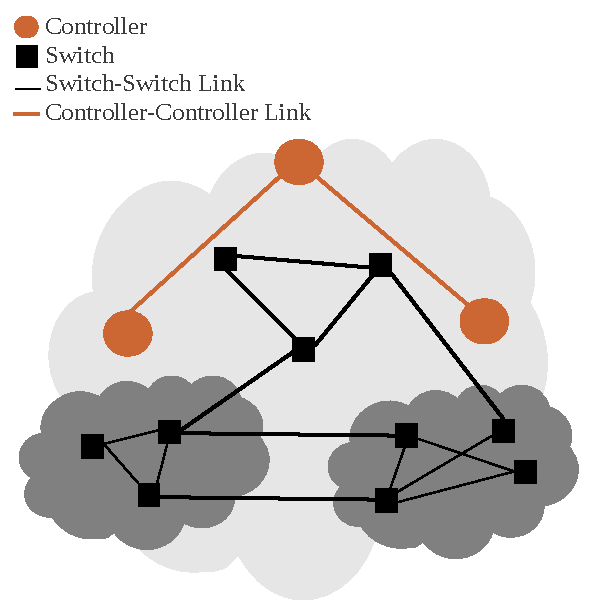
\includegraphics[scale=0.8]{network_view}
 \caption{A two-layer software defined network. The larger network contains two smaller networks and its controllers.}
 \label{fig:network_view}
 \end{figure}


However, the state of the entire network is distributed across different controllers. Hence, the controllers need to collaborate to perform invariant verification. Each update arriving on a slice' controller can have effects that are entirely local to the slice or not. Given a slice of network and a rule update that has effect only on that slice, verifying whether the update would cause any invariant violatations is a problem that has been studied. ~\cite{veriflownsdi},~\cite{netplumber} What is not obvious is how to determine whether the rule update affects any other slices in the network. In the next few sub-sections we present the outline of a design that answers this question. 

\subsection{Network Slices are Switches}

The key idea is to think of a network slice as an \textit{equivalent switch} with all its peering links as ports. The entire state contained by the controller can be expressed as rules on a switch expressing just what enters and what portion of the entering traffic exits various other ports while abstracting details of state related to intra-slice forwarding done by switches. This is accomplished by borrowing the technique presented by Peyman et. al. in NetPlumber ~\cite{netplumber}. The trick is to attach sources and sinks at all the peering interfaces to compute just what enters/exits that particular peer. Once that is computed, simplistic forwarding rules expressing the relationship between input and output traffic at each peering port can be computed.  Hence, each controller becomes just another switch containing these equivalent rules. This switch representation is initially formed and subsequently updated as verified rules are applied to the local slice' network.


 \begin{figure}[h]
 \centering
 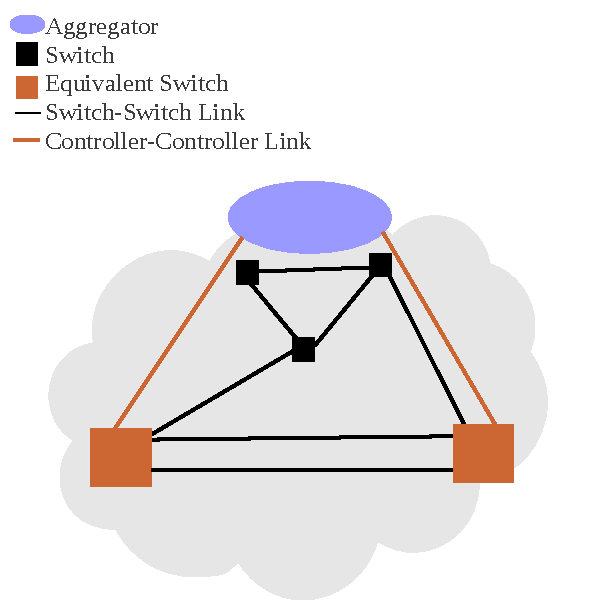
\includegraphics[scale=0.8]{alternative_network_view}
 \caption{An equivalent view of the network.}
 \label{fig:alternative_network_view}
 \end{figure}


\subsection{Aggregation Nodes}
Each controller shares its switch representation with one aggregation node. Each aggregating node collects switch representations from multiple controllers. Hence the aggregation nodes are essentially looking at a collection of switches and they can further do what individual controllers did and compress the state again to form a single switch representing the state of a collection of controllers and further share it with other aggregation nodes in other parts of the network. This design choice follows the SDN philosophy of converging state - which comes at the cost of introducing central points of failures in the network while making computation model simple and in this case more amenable to analysis. Also, this enables one to model an aggregation node essentially as just another controller.

\subsection{Rule Update Propagation}
When a rule update arrives at a particular controller, it first checks whether the rule does not put the local slice's network in an incorrect state. If not, then the controller creates an \textit{equivalent rule update} on its equivalent switch which represents the impact of applying the rule update on its network slice. It then forwards the equivalent rule update to the aggregation node which performs the same analysis \textit{locally} on the state that now spans multiple controllers. Since the aggregation node is just another controller, it can further replicate the operation that happened on the individual controller, i.e. to check if the rule update is 'local' or whether it needs to be forwarded further up to a higher level aggregation node. Hence the process keeps repeating until the equivalent update has propagated to all the aggregation nodes that it can potentially affect. 

\subsection{Rule Update Application}
When a rule update arrives at a controller, it has to wait for the update to propagate to all the aggregation nodes in the hierarchy and for the result to propagate back. Whether or not it violates any invariants can only be determined once all the results have been received by the entire hierarchy of aggregators. Our design choice is to wait until such determination is made before applying the update to the switches. This choice allows for the network to always be in the invariant conformant state at all times. However, we wish to study how long does \textit{on average} for such decision to be taken.


% An example of a floating figure using the graphicx package.
% Note that \label must occur AFTER (or within) \caption.
% For figures, \caption should occur after the \includegraphics.
% Note that IEEEtran v1.7 and later has special internal code that
% is designed to preserve the operation of \label within \caption
% even when the captionsoff option is in effect. However, because
% of issues like this, it may be the safest practice to put all your
% \label just after \caption rather than within \caption{}.
%
% Reminder: the "draftcls" or "draftclsnofoot", not "draft", class
% option should be used if it is desired that the figures are to be
% displayed while in draft mode.
%
%\begin{figure}[!t]
%\centering
%\includegraphics[width=2.5in]{myfigure}
% where an .eps filename suffix will be assumed under latex, 
% and a .pdf suffix will be assumed for pdflatex; or what has been declared
% via \DeclareGraphicsExtensions.
%\caption{Simulation Results}
%\label{fig_sim}
%\end{figure}

% Note that IEEE typically puts floats only at the top, even when this
% results in a large percentage of a column being occupied by floats.


% An example of a double column floating figure using two subfigures.
% (The subfig.sty package must be loaded for this to work.)
% The subfigure \label commands are set within each subfloat command, the
% \label for the overall figure must come after \caption.
% \hfil must be used as a separator to get equal spacing.
% The subfigure.sty package works much the same way, except \subfigure is
% used instead of \subfloat.
%
%\begin{figure*}[!t]
%\centerline{\subfloat[Case I]\includegraphics[width=2.5in]{subfigcase1}%
%\label{fig_first_case}}
%\hfil
%\subfloat[Case II]{\includegraphics[width=2.5in]{subfigcase2}%
%\label{fig_second_case}}}
%\caption{Simulation results}
%\label{fig_sim}
%\end{figure*}
%
% Note that often IEEE papers with subfigures do not employ subfigure
% captions (using the optional argument to \subfloat), but instead will
% reference/describe all of them (a), (b), etc., within the main caption.


% An example of a floating table. Note that, for IEEE style tables, the 
% \caption command should come BEFORE the table. Table text will default to
% \footnotesize as IEEE normally uses this smaller font for tables.
% The \label must come after \caption as always.
%
%\begin{table}[!t]
%% increase table row spacing, adjust to taste
%\renewcommand{\arraystretch}{1.3}
% if using array.sty, it might be a good idea to tweak the value of
% \extrarowheight as needed to properly center the text within the cells
%\caption{An Example of a Table}
%\label{table_example}
%\centering
%% Some packages, such as MDW tools, offer better commands for making tables
%% than the plain LaTeX2e tabular which is used here.
%\begin{tabular}{|c||c|}
%\hline
%One & Two\\
%\hline
%Three & Four\\
%\hline
%\end{tabular}
%\end{table}


% Note that IEEE does not put floats in the very first column - or typically
% anywhere on the first page for that matter. Also, in-text middle ("here")
% positioning is not used. Most IEEE journals/conferences use top floats
% exclusively. Note that, LaTeX2e, unlike IEEE journals/conferences, places
% footnotes above bottom floats. This can be corrected via the \fnbelowfloat
% command of the stfloats package.


\section{Model Description}
We simulate the model described above using the Python simulation package SimPy~\cite{simpy}. The network topology that we consider is that of hubs-and-spokes. Each spoke contains numerous switches and a controller. The controller in the spoke connects to a hub, where we assume an aggregation node is present. The aggregation node has multiple spokes' connecting to it. Furthermore, the aggregation node's network can then also behaves as a spoke to a larger network and so on. Hence the hub-and-spoke essentially reduces to a tree with multiple aggregation levels and an outdegree. All nodes except the leaves of this aggregation are aggregating controllers. The leaves are just simple controllers where updates are generated. 

\subsection{Parameters}
\begin{itemize}
 \item Exponentially Distributed Arrival Times: Each controller is responsible for producing updates. We use a single arrival generator to generate updates at a rate scaled by total number of controllers in the system and then splitting the arrivals using uniform distribution among all controllers.
 \item Exponentially Distributed Service Times: We assume the same service time distribution for all controllers and aggregators. 
 \item Probability of Hopping: The probability that when the update arrives on the controller/aggregator, it will be sent to the next. It is uniformly chosen and this makes the total number of aggregation layers that are involved in processing an update to be geometrically distributed.
 \item 
 
 \end{itemize}

\subsection{Metrics}
The key metric of interest is the Total Processing Time for any update. This is computed by keeping track of update's arrival on every hop and summing over processing times on all hops.

\subsection{Policies}
Our simulated system only has one policy of waiting before the arrival results come to apply the update. 

\section{Experimental Design}
We perform an $2^k$ factorial design over all the parameters described above.

\section{Conclusion}
In the previous study using analytic methods, we were limited by the state-space explosion when it came to obtaining results for larger topologies. The results of this study are same for smaller networks that could be analyzed using analytic methods and hence trustworthy to be extrapolated. 



% 
% \section{Model Description}
% We model from the perspective of a single \textit{incident} controller interacting with the hierarchy of aggregators, i.e. the controller at which updates are arriving. Each update would require a random number of aggregation levels to be travelled depending on just what traffic that rule update affects. At a given time, only one rule update is processed by the incident controller, i.e. it waits until the responses by all the aggregators have been received, then decides what to do about the rule update and then moves on to the next one.
% 
% 
%  \begin{figure}[h]
%  \centering
%  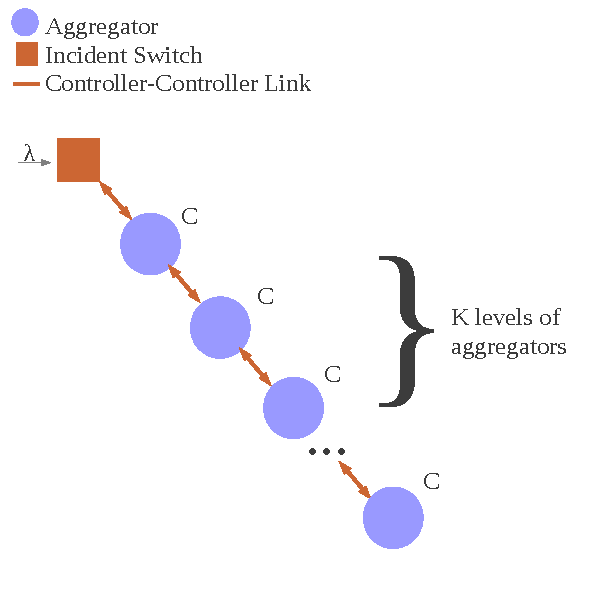
\includegraphics[scale=0.8]{model_perspective}
%  \caption{Perspective of the network that model takes.}
%  \label{fig:alternative_network_view}
%  \end{figure}
% 
% 
% 
% \subsection{Model Assumptions}
% 
% \begin {itemize}
%  \item Assume exponential arrival time distribution for rule update arrivals with the rate given by $\lambda$.
%  \item There are $K$ aggregation levels in the hierarchy of controllers, where $K$ is finite. 
%  \item The distribution of how many aggregation levels a given rule update triggers given by $n$ is a decreasing function. Intuitively, this is to express that rule updates affect the network topology in their local \textit{neighborbood} more often than they affect things in \textit{farther} places. The model uses a linearly decreasing function for this. So, $P(n_i) = mU(i) + b$, where $U(i)$ is the pdf of uniform distribution, $m$ is negative and its magnitude controls how fast the effect of an update dimnishes and $b$ is the baseline intercept.
%  \item Time spent on processing an update on any level is assumed to be constant and is given by $C$. Total time spent processing $n$ levels then is given by $nC$. Hence the service rate for a given update is given by $nC$. 
%  \item Size of the queue for holding updates is fixed is referred to as $B$.
%  
% %  
% %  \item Di is the degree parameter. It indicates for a given level i, how many sub-controllers can be directly calling it an aggregator. Canonically, Di is 0 for i = 1, but it can be random or a deterministic function of i.
% %  
% %  \item There are arrivals on each level of controller. Arrival rates are given by lambda i. Lambda is a function of (Di). 
% %  
% %  \item There are service rates for each level of aggregator. Service rates are given by $\mu_i$, for each aggregation level $i$. $\mu_i$ should be a function of $d_i$ to allow for scalable processing as one gets closer to the network core. We explore how linear of a function is this required to be for a stable queue.
% 
% \end {itemize}
% 
% \subsection{Model Rewards}
% 
% 
% \begin{itemize}
%  
%  \item \textbf{Expected wait time until service:} The average amount of time it takes for the results of verification of the rule update to propagate back towards the incident controller is given by $W$. With $L$ being the average number of rule updates in the queue waiting to be processed and $\lambda$ being the arrival rate,  little's law ~\cite{kleinrock} suggests:
%  
% \begin{equation*}
%  W = \frac{L}{\lambda}
% \end{equation*}
% 
% Assuming a fixed $\lambda$ on the incident controller and by associating a steady rate reward on the size of queue, one can compute $W$ for a given set of model parameters.
%  
% 
%  
%  
% \end{itemize}
% 
% 
% 
% \section{Results and Conclusion}
% 
% We implemented the model described above using Stochastic Activity Networks in Mobius. We solved the model for various values of $m$, $\lambda$ and $C$. The results for the same are presented in figures \ref{fig:incident_isss_positive_slope},  \ref{fig:incident_isss_zero_slope} and \ref{fig:incident_isss_negative_slope}. As evident, as the slope decreases, the system scales better, which is easily explained by the fact that decrease in slope indicates fewer queries generated for processing to distant controllers. It is not clear what slopes in the real networks look like, however several recent studies have made arguments for it to be negative. 
%  
% 
%  \begin{figure}[h]
%  \centering
%  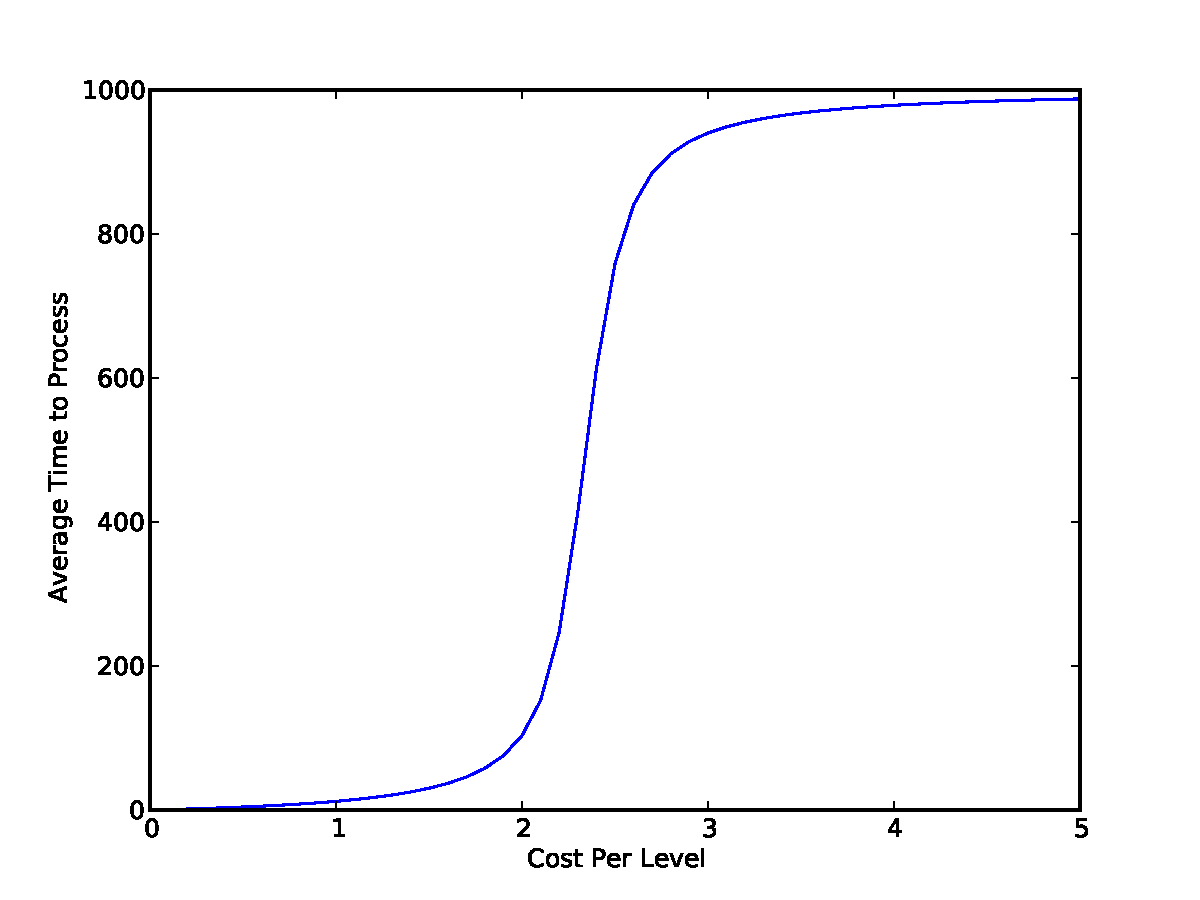
\includegraphics[scale=0.50]{incident_isss_positive_slope}
%  \caption{Design scaling when m = 1}
%  \label{fig:incident_isss_positive_slope}
%  \end{figure}
% 
%  
%  Furthermore, all the curves exhibit a knee, which is characteristic of a bounded-queue system. This indicates presence of a tipping point, which once reached, can potentially send the system in to chaos. However as the slope decreases, one observes the knee being displaced towards right, which indicates that the tipping point becomes less likely to be hit.
%  
%  \begin{figure}[h]
%  \centering
%  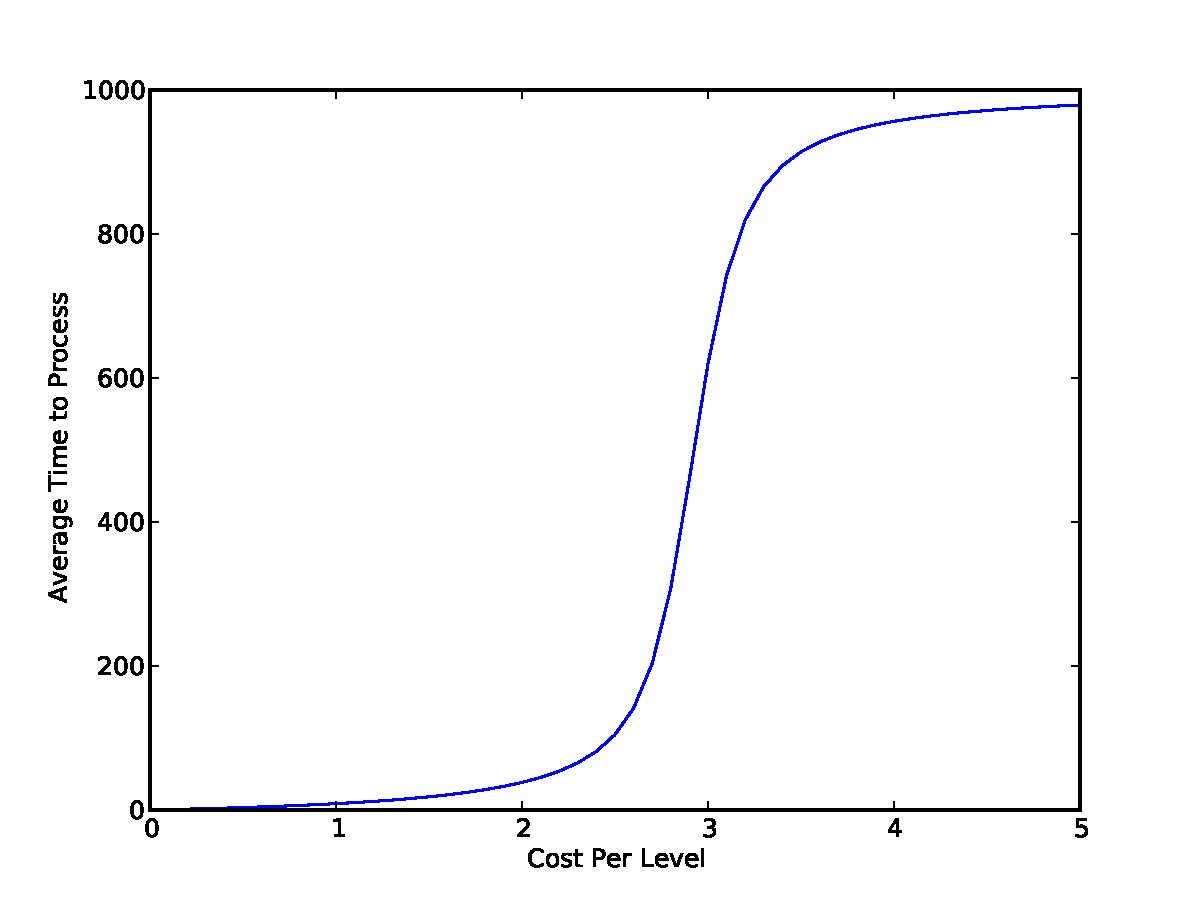
\includegraphics[scale=0.50]{incident_isss_zero_slope}
%  \caption{Design scaling when m = 0}
%  \label{fig:incident_isss_zero_slope}
%  \end{figure}
% 
%  And finally, the magnitude of average time required to process an update decreases with slope and increases with per-level costs. Since we assumed fixed costs per level, this view is simplistic. This suggests that as one gets closer to the core of network, there is potential for improved performance if the cost is reduced per aggregation level.
% 
%  \begin{figure}[h]
%  \centering
%  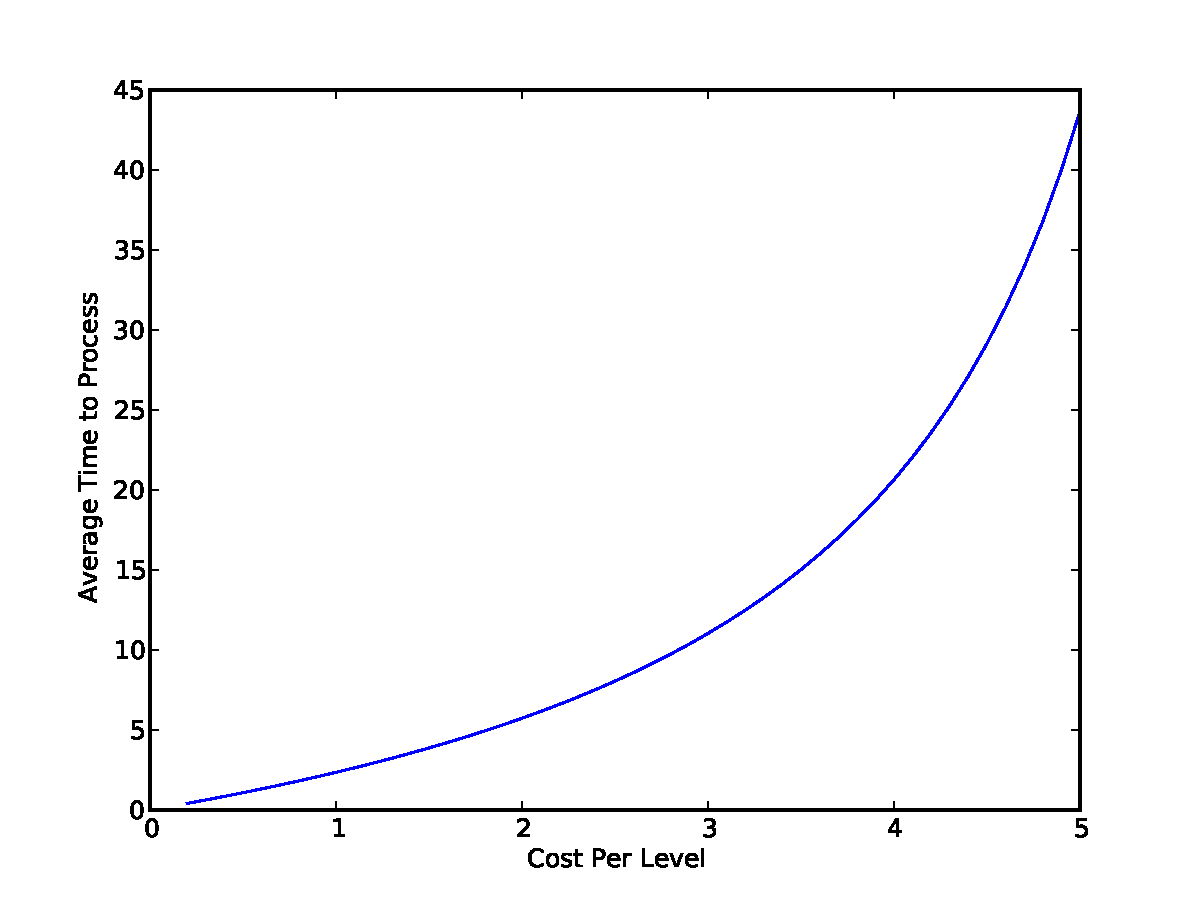
\includegraphics[scale=0.50]{incident_isss_negative_slope}
%  \caption{Design scaling when m = -1}
%  \label{fig:incident_isss_negative_slope}
%  \end{figure}
% 
% 
% \section{Future Work}
% The model studied here is very simple but it captures the dynamics of the system. It also provides some design insights into potentially allowing parallel updates and rolling back if they fail to pass. Performance of studying such system would be one future direction this model can be extended towards. One can also study and quantify the cost of consistency in the face of higher workloads and derive trade-offs for real systems by modelling more complex dyanmics of the design.

% conference papers do not normally have an appendix
% 
% 
% % use section* for acknowledgement
% \section*{Acknowledgment}
% 
% 
% The authors would like to thank...





% trigger a \newpage just before the given reference
% number - used to balance the columns on the last page
% adjust value as needed - may need to be readjusted if
% the document is modified later
%\IEEEtriggeratref{8}
% The "triggered" command can be changed if desired:
%\IEEEtriggercmd{\enlargethispage{-5in}}

% references section

% can use a bibliography generated by BibTeX as a .bbl file
% BibTeX documentation can be easily obtained at:
% http://www.ctan.org/tex-archive/biblio/bibtex/contrib/doc/
% The IEEEtran BibTeX style support page is at:
% http://www.michaelshell.org/tex/ieeetran/bibtex/
%\bibliographystyle{IEEEtran}
% argument is your BibTeX string definitions and bibliography database(s)
%\bibliography{IEEEabrv,../bib/paper}
%
% <OR> manually copy in the resultant .bbl file
% set second argument of \begin to the number of references
% (used to reserve space for the reference number labels box)
\begin{thebibliography}{1}

\bibitem{openflow}
Nick McKeown, Tom Anderson, Hari Balakrishnan, Guru Parulkar, Larry Peterson,
  Jennifer Rexford, Scott Shenker, and Jonathan Turner.
\newblock Openflow: enabling innovation in campus networks.
\newblock {\em SIGCOMM Comput. Commun. Rev.}, 38(2):69--74, March 2008.


\bibitem{veriflownsdi}
Ahmed Khurshid, Xuan Zou, Wenxuan Zhou, Matthew Caesar, and Brighton Godfrey.
\newblock Veriflow: Verifying network-wide invariants in real time.
\newblock In {\em Proceedings of the 10th USENIX conference on Networked
  Systems Design and Implementation}, NSDI'13, 2013.


\bibitem{netplumber}
Peyman Kazemian, Michael Chang, Hongyi Zeng, George Varghese, Nick McKeown, and
  Whyte. Scott.
\newblock Real time network policy checking using header space analysis.
\newblock In {\em Proceedings of the 10th USENIX conference on Networked
  Systems Design and Implementation}, NSDI'13, 2013.
  

\bibitem{tcpp}
Brandon Heller, Rob Sherwood, and Nick McKeown.
\newblock The controller placement problem.
\newblock In {\em Proceedings of the first workshop on Hot topics in software
  defined networks}, HotSDN '12, pages 7--12, New York, NY, USA, 2012. ACM.
  

\bibitem{mcleod}
Bruce~Daniel McLeod.
\newblock Performance analysis of n-processor time warp using stochastic
  activity networks.
\newblock Master's thesis, University of Arizona, 1993.
  

\bibitem{kleinrock}
Kleinrock, Leonard
\newblock Queueing systems. volume 1: Theory
\newblock 1975, Wiley-Interscience

\bibitem{simpy}
Muller, Klaus
\newblock Advanced systems simulation capabilities in SimPy
\newblock Europython, 2004.

  
\end{thebibliography}






% that's all folks
\end{document}


